\documentclass{article} % For LaTeX2e
\usepackage{nips13submit_e,times}
\usepackage{graphicx}
\usepackage{hyperref}
\usepackage{url}
%\documentstyle[nips13submit_09,times,art10]{article} % For LaTeX 2.09


\title{Localizing a SCUBA Diver Using Active Sonar}


\author{
Richard Guilmain \\
Georgia Tech\\
\texttt{rguilmain@gatech.edu} \\
\And
Nabin Sharma \\
Georgia Tech\\
\texttt{nsharma@gatech.edu} \\
}

% The \author macro works with any number of authors. There are two commands
% used to separate the names and addresses of multiple authors: \And and \AND.
%
% Using \And between authors leaves it to \LaTeX{} to determine where to break
% the lines. Using \AND forces a linebreak at that point. So, if \LaTeX{}
% puts 3 of 4 authors names on the first line, and the last on the second
% line, try using \AND instead of \And before the third author name.

\newcommand{\fix}{\marginpar{FIX}}
\newcommand{\new}{\marginpar{NEW}}

\nipsfinalcopy % Uncomment for camera-ready version

\begin{document}


\maketitle

%% \begin{abstract}
%% \end{abstract}

\section{Problem Description}
The threat of an underwater terrorist attack is a concern of the maritime industry,
port law enforcement, and luxury and high-profile vessel owners alike. Prevention of
such attacks needs to start with the reliable detection of sub-surface threats such
as SCUBA and closed-circuit re-breather (CCR) divers. Because these threats are below
the water’s surface, traditional detection methods such as radar and visual surveillance
are unavailable, making active sonar technology the most effective approach to date.
However, because of the inherent noise of the underwater acoustic environment—often
rife with mechanical noise, reflective debris, and environmental marine activity—current
sonar methods are often inconsistent. Better processing methods are required to manage
this low signal-to-noise ratio while still localizing the range and bearing of
threatening divers at tactically significant ranges.

Given the noisy range and bearing measurements from an active sonar receiver, the goal
is to estimate the range of the target to the sensor, the bearing of the target to the sensor,
and the heading direction that the target is moving in. Due to relatively unstable
propagation environment, underwater targets like SCUBA divers might not be detected
for all measurement steps even if relatively noisier measurements are accepted as valid
ones. This leads to the requirement of more robust localization schemes so that we don't
lose valid targets just because we missed corresponding measurements intermittently.

\begin{figure}
  \centering
  \fbox{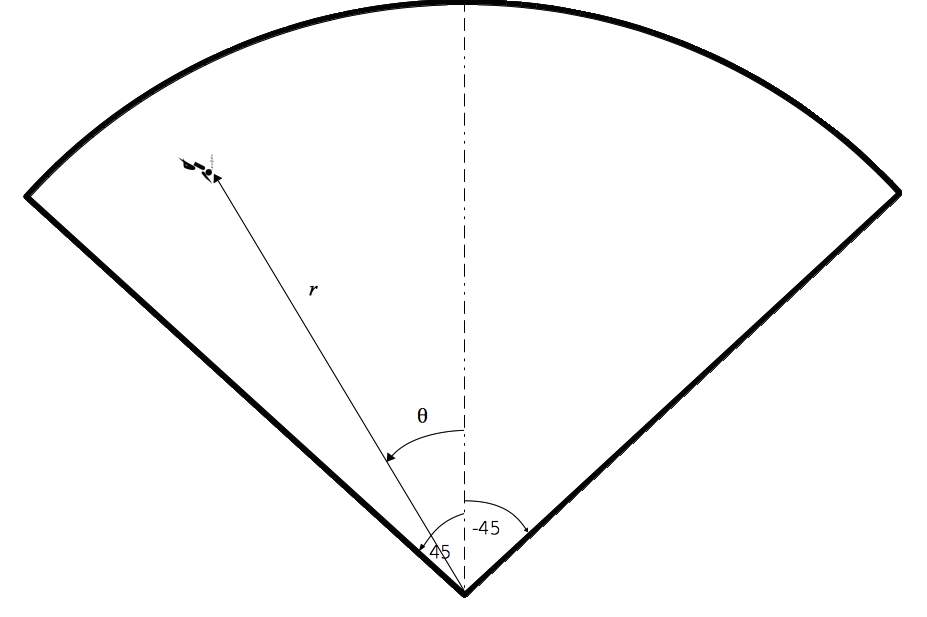
\includegraphics[width=0.9\textwidth]{sector.png}}
  \caption{Basic graphical representation of a typical diver localization scenario. Sonar
    measurements provide the range ($r$) of the target (or diver) from the sonar sensor and
    bearing ($\theta$) from the sonar sensor axis represented by dashed line. The angular
    span of the sensor field-of-view is $90^{\circ}$.}
  \label{fig:sector_cartoon}
\end{figure}

\begin{figure}
  \centering
  \fbox{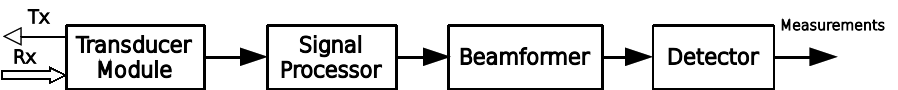
\includegraphics[width=0.9\textwidth]{blocks.png}}
  \caption{Block diagram of the active sonar receiver used to obtain diver measurements.}
  \label{fig:blocks}
\end{figure}

\begin{figure}
  \centering
  \fbox{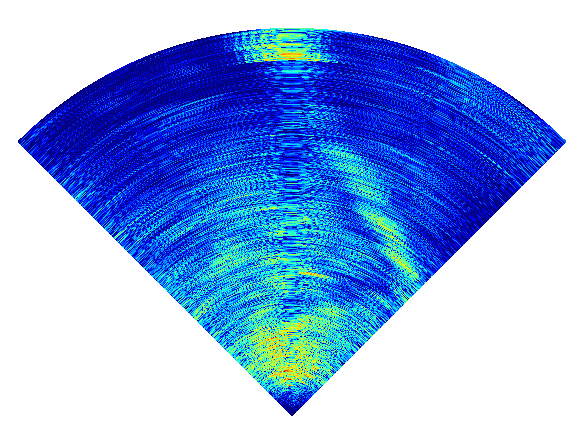
\includegraphics[width=0.9\textwidth]{sector_example.png}}
  \caption{A representative sonar sector. As shown in Fig.~\ref{fig:sector_cartoon}, the
    sonar field-of-view is $90^{\circ}$ and maximum range is 500 meters. The relatively
    stronger patch at around $0^{\circ}$ and 450 meters is diver.}
  \label{fig:sector_example}
\end{figure}

\section{Sensor and Measurements}
Figure \ref{fig:sector_cartoon} shows a typical diver localization scenario. Center of the sector
in Fig.~\ref{fig:sector_cartoon} represents
the location of active sonar sensor in a ship or boat in a water surface.  The sonar system is
responsible for providing measurements to our diver localization algorithm. The sonar transmits
an acoustic pulse every $1.3$ seconds and listens for echo returns via a multichannel receive array.
Fig.~\ref{fig:blocks} shows the signal and data processing block diagram of the sonar system. Data from receive
array passes through several signal processing modules, for example, lowpass filer, digital
downconverter, etc., before it gets ready for beamforming. During beamforming, the sonar software
combines the signals from all receive array channels in a controlled manner so that the difference
time delays experienced by sonar echoes to enter the different receive channels is equalized for
desired directions along which sonars want to look for targets. This effectively increases the
receiver gain in the desired directions and thus helps in getting better diver or target
measurements.

As shown in Fig.~\ref{fig:sector_cartoon}, we set the sonar, specifically, the beamformer, to look for 45 degrees
on both sides of sonar axis. This sets the sonar angular field-of-view to be of $90^{\circ}$.
The maximum range up to which the sonar can detect the target is $500$ meters. The angular
field of view and the maximum detection range of the sonar define the sonar sector as
shown in Fig.~\ref{fig:sector_cartoon} - the only area in front of sonar which can be scanned for detecting
targets. Fig.~\ref{fig:sector_example} shows a sector generated using the range and angular settings as
specified in Fig.~\ref{fig:sector_cartoon}. The relatively strong patch around $0^{\circ}$ and $450$ meters
is a SCUBA diver swimming towards the sonar. It is evident from Fig.~\ref{fig:sector_example} that the sector
data coming out of beamformer could be quite noisy depending on the conditions of water
and surroundings. We have to accept some level of false detections to have true measurements
from diver. This leads to the requirement of a probabilistic localization algorithm if we
want to detect the diver with high level of confidence.

The detector itself in Fig.~\ref{fig:sector_cartoon} tries to minimize the effects of noise and false detections
as much as possible without losing the true target measurements. As explained before, the
detector in Fig.~\ref{fig:blocks} takes sonar beams like in Fig.~\ref{fig:sector_cartoon} as input. It then implements several
signal and data processing algorithms to suppress unmoving targets, noise and interference
from other sound sources under water. The detector implements ping-to-ping exponential
smoothing and background subtraction algorithms to provide relatively cleaner moving targets
measurements to localization algorithm. The targets that are of most importance are the ones
moving towards the ship or sonar. So the detector is tuned to detect targets that are moving
radially towards the sonar sensor more effectively than the targets moving otherwise.

\section{Conclusion}

\section*{Acknowledgments}

\end{document}
